\graphicspath{{./fig_DH/}}
%

\hypertarget{tgt:DH}{\section{時系列データ保持機能}}

時系列データ保持機能では,
ソルバー実行開始時に,指定されたファイル(入力データファイル)より
時系列データ(データセット)を読み込み,
ソルバー実行中にその値を参照できる機能を提供する.

入力データセットは時系列だけでなく,速度値に対する圧力損失値のように,
定義域が時間以外の物理量の場合にも対応可能である.
以下では便宜上,参照時にキーとなる量を「時刻」,参照したい量を「値」
と記すことにする.

データ値は,入力データセット毎に付けられたラベルと,時刻をキーにして
以下の規則により参照される.
\begin{itemize}
\item[-] 指定された時刻のデータがデータセット内に存在した場合,その時刻での値
\item[-] 指定された時刻がデータセット内の最小時刻より小さい場合,最小時刻データの値
\item[-] 指定された時刻がデータセット内の最大時刻より大きい場合,最大時刻データの
値
\item[-] その他の場合,指定された時刻を挟む2つの時刻データから,線形補間により値を計算
\end{itemize}



\subsection{XMLコンフィギュレーションファイルによる入力データファイル指定方法}
XMLコンフィギュレーションファイルのParameterセクションの
Data\_Holder要素内に,データセット数分のParam要素を記述する.
各Param要素には,name属性にデータの内容を表すラベル文字列を,
文字列型のvalue属性にデータファイルのパスを指定する.
ソルバー内部では,このラベル文字列によりデータセットの識別を行う.
{\small
\begin{program}
<Parameter>
  …
  <Elem name="Data_Holder">
    <Param name="label1" dtype="STRING" value="data/data1.dat" />
    <Param name="label2" dtype="STRING" value="data/data2.dat" />
  </Elem>
  …
</Parameter>
\end{program}
}
上例では,dataディレクトリの2つのデータファイルdata1.dat, data2.datを,
それぞれ「label1」「label2」というラベルを付けて指定している.


\subsection{入力データファイルのフォーマット}
入力データファイルは,テキストファイルとし,
各行に一組ずつ時刻と値を次の規則に従って記述する.
\begin{itemize}
\item[-] 時刻と値は,空白またはカンマで区切るものとする.
\item[-] 空白とは1つ以上の,半角スペースまたはタブである.
\item[-] 時刻の前,値の後ろ,カンマの前後に,空白を入れることもできる.
\item[-] 空行および「{\tt \#}」で始まるコメント行を任意の場所に挿入できる.
\item[-] 時刻と値の後ろに,さらに空白またはカンマを挟んでレコードが続く場合,
それらは無視される.
\end{itemize}
なお,時刻は昇順にソートされている必要はないが,同一時刻のデータが複数存在する場合にはエラーとして扱い,ソルバーの実行を停止する.

{\small
\begin{program}
#
# 1行に2つの実数「時刻」と「値」を空白またはカンマ区切りで記述
#
  時刻1   値1  # 空白区切り
  時刻2,値2    # カンマ区切り
  時刻3,  値3  # カンマ+空白区切り
   …       …
  時刻n   値n
\end{program}
}

\subsection{API説明}
時系列データ保持機能は,
個々のデータセットの内容を保持管理するDataHolderクラスと,
DataHolderクラス全体を管理するDataHolderManagerクラスからなる.
なお,DataHolderManagerクラスは,Parallel\_Nodeクラスから継承されている.
\begin{figure}[H]
\vspace{0.5cm}
\begin{center}
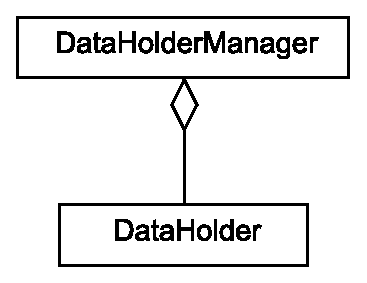
\includegraphics[width=0.18\textwidth]{DataHolder.eps}
\caption{時系列データ保持機能 クラス図}
\label{fig:data_holder}
\end{center}
\end{figure}

\subsubsection{DataHolderManagerクラス公開メソッド}

\paragraph{DataHolderの取得}\mbox{}\\
ラベル{\tt label}を指定して,対応するデータセットを保持管理している
DataHolderクラスオブジェクトへのポインタを返す.
対応するデータセットがない場合には0を返す.
{\small
\begin{program}
DataHolder* getDataHolder(const string& label)
\end{program}
}

\paragraph{DataHolder数の取得}\mbox{}\\
管理下にあるDataHolder数を返す.
{\small
\begin{program}
unsigned getNumDataHolder() const
\end{program}
}

\paragraph{DataHolder情報の出力}\mbox{}\\
管理下にある全DataHolderの情報を出力する.
{\small
\begin{program}
void printInfo(FILE* fp) const
\end{program}
}

\paragraph{DataHolder情報の出力(デバッグ用)}\mbox{}\\
管理下にある全DataHolderの情報(全データ内容を含む)を出力する.
{\small
\begin{program}
void printInfoDebug(FILE* fp) const
\end{program}
}

\paragraph{XMLファイルポインタの受け取り}\mbox{}\\
XMLコンフィギュレーションファイル({\tt SklCfg::SklSolverConfig}クラス)への
ポインタを受け取る.ポインタの内容が不正な場合,falseを返す.
{\small
\begin{program}
bool receiveCfgPtr(SlkCfg::SklSolverConfig* cfg)
\end{program}
}

\paragraph{データファイル読み込み}\mbox{}\\
XMLコンフィギュレーションファイルをパースし,入力データファイルを読み込み,
内部にDataHolderを生成し登録する.
{\small
\begin{program}
void readData()
\end{program}
}

\subsubsection{DataHolderクラス公開メソッド}
\paragraph{時刻を指定して値を取得}\mbox{}\\
指定された時刻{\tt t}に対して,格納データを参照して,線形補間により求めた値を返す.
指定された時刻が入力データの定義域外の場合には,最初あるいは最後の(最も近い時刻での)値を返す.
{\small
\begin{program}
SKL_REAL getValue(SKL_REAL t) const
SKL_REAL get_value(SKL_REAL t) const
\end{program}
}

\paragraph{データ値のスケーリング}\mbox{}\\
指定された倍率で,全時刻での値をスケーリングする.
データ値の単位変換などでの使用を想定している.
{\small
\begin{program}
void scale(SKL_REAL ratio)
\end{program}
}

\paragraph{時刻の最小値・最大値の取得}\mbox{}\\
時刻(データの定義域変数)の最小値・最大値を返す.
{\small
\begin{program}
SKL_REAL getMin() const
SKL_REAL getMax() const 
\end{program}
}

\paragraph{格納データ情報の出力}
格納データ情報(ラベル,ファイル名,データ数,時刻の最小値・最大値)を出力する.
{\small
\begin{program}
void printInfo(FILE* fp) const
\end{program}
}

\paragraph{格納データ情報の出力(デバッグ用)}
全格納データを出力する.
{\small
\begin{program}
void printInfoDebug(FILE* fp) const
\end{program}
}



\subsection{ソルバーへの組み込み方法}
DataHolderクラスおよびDataHolderManagerクラスを利用するには,
ヘッダファイルDataHolder.hをインクルードする必要がある.

\paragraph{初期化}\mbox{}\\
以下の4ステップが必要:
\begin{enumerate}
\item インスタンス化
\item setParallelInfoメソッドによる並列情報の設定
\item receiveCfgPtrメソッドによるXMLコンフィギュレーションファイルポインタの設定
\item readDataメソッドによる入力データファイルの読み込み
\end{enumerate}
\begin{program}
  Parallel_Info pn;
  SklCfg::SklSolverConfig* m_solvCfg;
  …
  // (1) インスタンス化
  DataHolderManager DH;   
  …
  // (2) 並列情報設定
  DH.setParallelInfo(pn);

  // (3) XMLコンフィギュレーションファイルポインタ設定
  if (!DH.receiveCfgPtr(m_solvCfg)) assert(0);

  // (4) 入力データファイル読み込み
  DH.readData();
\end{program}

\paragraph{データセットの参照}\mbox{}\\
以下の例のように,DataHolderクラスのポインタ変数を通して使う.
\begin{program}
  DataHolderManager DH;
  …
  /* ここでDHの初期化 */
  …
  // データセット「label1」へのポインタを取得
  DataHolder* data1 = DH.getDataHolder("label1");

  // エラー処理
  if (!data1) {
    printf("Error: no DataHolder labeled 'label1'.\n");
    …
  }

  SKL_REAL t = …;  // 時刻

  // 時刻tでの値を取得
  SKL_REAL x = data1->getVal(t);
\end{program}

また,次の例のように,DataHolderManagerのみを通して使うことも可能.
{\small
\begin{program}
  DataHolderManager DH;
  …
  /* ここでDHの初期化 */
  …
  SKL_REAL t = …;  // 時刻

  // データセット「label1」の時刻tでの値を取得
  SKL_REAL x = DH.getDataHolder("label1")->getVal(t);
\end{program}
}
